\documentclass[tikz,border=10pt]{standalone}


\begin{document}
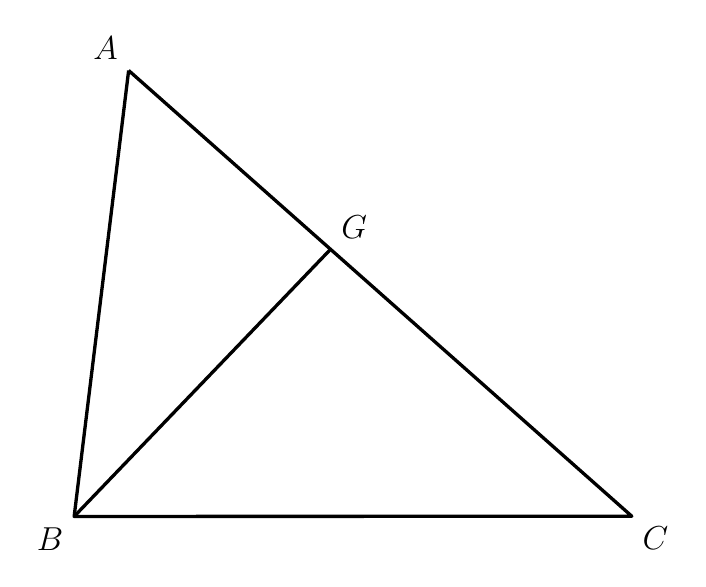
\begin{tikzpicture}[line width=1.2pt, line join=round]
\coordinate (A) at (-2.847,2.837);
\coordinate (B) at (-3.539,-2.827);
\coordinate (C) at (3.543,-2.824);
\coordinate (G) at (-0.283,0.566);

  
  \draw (A) -- (B) -- (C) -- (G) -- (A);
  
  \draw (B) -- (G);
  
  \node[above left] at (A) {\fontsize{13}{15.6}\selectfont $A$};
  \node[below left] at (B) {\fontsize{13}{15.6}\selectfont $B$};
  \node[below right] at (C) {\fontsize{13}{15.6}\selectfont $C$};
  \node[above right] at (G) {\fontsize{13}{15.6}\selectfont $G$};
\end{tikzpicture}
\end{document}